\documentclass[border=3pt,tikz]{standalone}
% Shared look for every TikZ figure in these notes.
% Included by each standalone figure file; also keeps the figures consistent
% with the colours used in the PDF and on the website.

\usepackage{tikz}
\usepackage{pgfplots}
\pgfplotsset{compat=1.18}
\usetikzlibrary{arrows.meta, decorations.markings, decorations.pathmorphing,
                patterns, calc, positioning}
\usepackage{amsmath}

% Series colours are the three validated categorical slots also used by the
% interactive widgets, so a path drawn in the printed notes and the same path on
% the website are the same colour. They clear the colour-vision-deficiency and
% contrast checks as a set; every path is direct-labelled as well, so colour is
% never the only thing carrying identity.
\definecolor{duPurple}{HTML}{68246D}
\definecolor{duBlue}{HTML}{2A78D6}
\definecolor{duRed}{HTML}{EB6834}
\definecolor{duGreen}{HTML}{1BAF7A}
\definecolor{duGrey}{HTML}{6B6B6B}

\tikzset{
  axisline/.style   = {-{Stealth[length=3mm]}, line width=0.7pt, black},
  path1/.style      = {duBlue,   line width=1.1pt},
  path2/.style      = {duRed,    line width=1.1pt},
  path3/.style      = {duGreen,  line width=1.1pt},
  statedot/.style   = {circle, fill=black, inner sep=1.4pt},
  arrowhead/.style  = {decoration={markings,
                        mark=at position #1 with {\arrow{Stealth[length=2.6mm]}}},
                       postaction={decorate}},
  lbl/.style        = {font=\small},
  slbl/.style       = {font=\footnotesize, duGrey},
  workfill/.style   = {duPurple, opacity=0.16},
}

% Textbook power-plant schematic (655 x 456 px) with the board labels on top.
\newcommand{\pxs}{0.0125}
\newcommand{\px}[2]{({#1*\pxs},{(456-#2)*\pxs})}
\begin{document}
\begin{tikzpicture}
  \node[anchor=south west, inner sep=0] at (0,0)
    {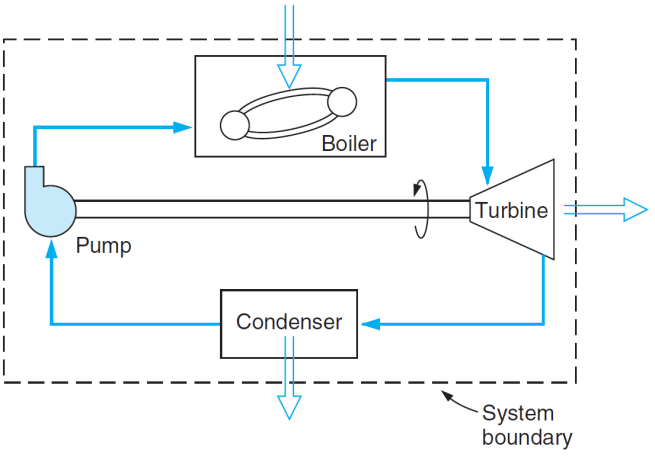
\includegraphics[width=8.1875cm]{../img/ch5-power-plant-img.png}};
  \node[anchor=west, text=duRed, font=\normalsize] at \px{300}{18}
    {$\dot{Q}_\text{boiler} > 0$};
  \node[anchor=south, text=duGreen!80!black, font=\normalsize] at \px{625}{180}
    {$\dot{W} < 0$};
  \node[anchor=east, text=duBlue, font=\normalsize] at \px{275}{415}
    {$\dot{Q}_\text{con} < 0$};
  \draw[-{Stealth[length=2.6mm]}, line width=1.3pt, duGreen!80!black]
    \px{455}{190} -- \px{215}{190};
\end{tikzpicture}
\end{document}
